
\chapter{Introduction}

%We explore the available formalisms for design of asynchronous digital
%circuits and compare them with the principle of compositionality in
%mind. We propose improvements to the existing techniques and
%propose a new formalism, Parametrised Graph (PG) theory, which is a
%generalisation of the existing CPOG formalism. We furhter study 
%the theory of PG Algebra and present mechanised formal proofs of certain properties.


% productivity gap
The major challenge for the future of semiconductor industry is the infamous design productivity gap. This gap is caused by the exponential complexity growth of electronic systems~\cite{Moore_1965_e}  while capability of design tools cannot cope with this pace, see Fig.~\ref{fig:productivity_gap}. The only way to deal with the increasing complexity of Integrated Circuits (ICs) is to improve the efficiency of the design process, in particular, by heavily reusing system components and by advancing the design automation methods.

\begin{figure}
\centering
  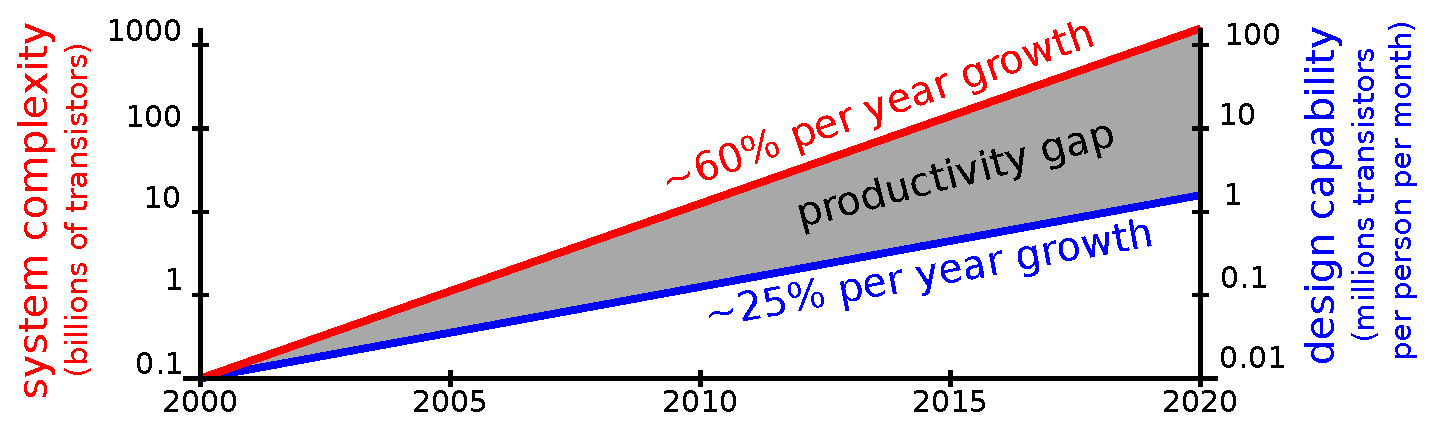
\includegraphics[scale=0.5]{fig/figs/productivity_gap}
  \caption{
    \label{fig:productivity_gap}
    Desigh productivity gap}
\end{figure}


% design reuse and need for async design principles
It has been predicted by ITRS~\cite{ITRS_2011} that in order to address the productivity gap challenge, by 2020 at least 90\% of the complex circuits should be built of previously designed components. This rises the need for compositional (or modular) design principles where the timing of individual modules is independent of the rest of the system and  therefore require delay insensitive communication between the modules. This communication discipline is natural for asynchronous circuits where the data transition is accompanied by request-acknowledgement handshaking between the sending and the receiving counterparts. On this pathway the previously designed Intellectual Property (IP) cores will need to be adapted to the new modular architectures. The least intrusive is the Globally Asynchronous Locally Synchronous (GALS) approach~\cite{Chapiro_1984_phd} where special wrappers~\cite{Mullins_2007_async, Fan_2009_iccd} are built around synchronous modules to convert their communication into asynchronous handshake style. Another alternative is desynchronisation techniques~\cite{Cortadella_2006_ieeetcad} where the global clock is replaced by a distributed control which determines when the computation is complete and the output result is ready to be consumed. This control may take different forms, from a delay line matching the critical path of the module~\cite{Cortadella_2010_icicdt } to explicitly introduced completion detection logic~\cite{Kondratiev_2002_ieeedtc}.

% synthesis of async components
The remaining 10\% of the ICs will still need to be designed from scratch. One way is to design those components in traditional synchronous way and then apply the previously discussed techniques to comply with the delay insensitive interface requirements. This, however, may result in suboptimal solutions in terms of circuit area, computation speed and energy consumption. Better results can be achieved if the components are designed and implemented with their asynchronous environment in mind~\cite{Martin_2006_ieeeproc}. However, the logic synthesis of asynchronous circuits is computationally expensive and not applicable to large modules. This is due to high level of concurrency in truly asynchronous systems which results in a state space explosion.  The computation complexity problem has been successfully addressed in the syntax-driven translation~\cite{Tangram-or-Balsa-paper?} approach which is based on direct mapping of specification into hardware components without going through the state space exploration (it is assumed that there is one-to-one correspondence between the specification language constructs and the library of available components).

% need for compositional approach
The major drawback of the circuits obtained by the syntax-driven translation is the suboptimal performance of their control structures~\cite{Balsa-related-paper}. In order to resolve this issue the control models of all the components need to be composed together and resynthesised exploiting the benefits of their joint optimisation. Existing resynthesis methods are based on parallel composition of component models expressed in form of Petri nets~\cite{Desij-related-paper}. However, the efficient parallel composition of the component models is still an open question and is one of the primary goals of this thesis.

\begin{figure}
\centering
  \newcommand{\figgg}[2]{
    \subfloat[#1]{
      \label{fig:#2}
      \includegraphics[scale=0.7]{fig/figs/#2}
  }}
  \figgg{Structural composition}{composition_structural}
  \\
  \figgg{Naive behavioural composition}{composition_behavioural_naive}
  \figgg{Behavioural composition}{composition_behavioural}
  \caption{
    \label{fig:productivity_gap}
    Desigh productivity gap}
\end{figure}

% structural and behavioural aspects of composition
The composition of circuit components is of structural nature - they are combined via input-output interfaces according to the casual dependency between the operation they perform, as shown in Fig.~\ref{fig:composition_structural}.
Another compositional aspect is a combination of several mutually exclusive behaviours in the same circuit. A naive way to build such a circuit is to implement the different behaviour scenarious in separate modules and structurally compose them with the use of multiplexers and demultiplexers, as shown in Fig.~\ref{fig:composition_behavioural_naive}. A mode selection code on the (de)multiplexors determines the current scenario.  While this is a valid implementation of multi-modal functionality, it ignores the mutually exclusive feature of the implemented behaviours and looses a possibility of partial hardware reuse for common functionality, as shown in Fig.~\ref{fig:composition_behavioural}. 

A model which naturally captures the structural and behavioural aspects of composition in a single formalism is Conditional Partial Order Graphs (CPOGs)~\cite{Mokhov_2009_phd}. This graph-based model is capable of expressing the structural composition by means of causality arcs (similar to Petri nets) and the behavioural composition by means of boolean "visibility" conditions on its vertices. While CPOGs is a convenient tool for reasoning on small benchmarks, it lacks the means for capturing and transformation of large systems. An ambitious goal of this thesis is to generalise the CPOGs model and introduce a theory for their manipulation in algebraic form, which is a more suitable representation for complex benchmarks.



%\section{Motivation}
%
%With constantly growing transistor counts and consumer demands, the complexity of digital circuits must grow too.
%
%With the rising complexity of digital circuits, it becomes increasingly important to reuse parts of existing designs.
%
%The reuse of the components must be facilitated by the design language.
%
%One of the difficulties in designing modern hardware systems is the
%necessity to comprehend and to deal with a very large number of system
%configurations, operational modes, and behavioural scenarios. 
%
%\subsection{Compositionality}
%
%The key property facilitating component reuse is compositionality.
%
%Compositionality is a property of a given language where the meaning of a language construct is determined by the meanings of its parts.
%

\section{Contributions}

The main contributions of the thesis are as follows:

\begin{itemize}
\item
\textbf{Improved parallel composition:} a novel method for composition of models specified with labelled Petri Nets.

\item
\textbf{Balsa circuit synthesis:} application of labelled Petri nets and parallel composition to synthesis of Balsa handshake circuits.

\item
\textbf{CPOG Synthesis:} a technique for synthesis of processor instruction decoder using instruction sets specified with Conditional Partial Order Graphs.

\item
\textbf{PG theory:} formal specification of theory of parameterised graphs with CPOGs as an example of its algebra.

\item
\textbf{CAD tool support:} automation for design of CPOGs and Balsa circuits using Workcraft framework.

\end{itemize}

\section{Structure}

The rest of the thesis is organised as follows:

Chapter~\ref{chap:Background} covers the basics of handshake circuits, signal transition graphs and conditional partial order graphs.

Chapter~\ref{chap:Approach} overviews the existing composition methods and outlines the drawbacks using an intuitive GCD benchmark as an example.

Chapter~\ref{chap:ParComp} describes the proposed improved parallel composition algorithm.  .

Chapter~\ref{chap:PGAlgebra} introduces Parametrised Graph (PG) theory, defining and studying an algebraic structure that generalises Conditional Partial Order Graph formalism.

Chapter~\ref{chap:PGEncoding} describes a technique for optimal encoding of processor instruction sets defined using CPOG formalism.

Chapter~\ref{chap:Conclusion} summarises the achieved results and proposes ideas for future research.

